\documentclass[runningheads]{llncs}

\usepackage{iftex}
\ifPDFTeX
  \PackageError{short}{This manuscript must be built with XeLaTeX}{}
\else
  \usepackage{fontspec}
\fi
\usepackage{amsmath,amssymb}
\usepackage{booktabs}
\usepackage{graphicx}
\usepackage{xcolor}
\usepackage[hidelinks]{hyperref}
% Use the standard algorithm packages when available.  The compact fallback
% keeps this manuscript buildable on minimal TeX Live images; it is bypassed
% automatically on Overleaf and other installations that provide the packages.
\IfFileExists{algorithm.sty}{%
  \usepackage{algorithm}%
}{%
  \usepackage{float}%
  \newfloat{algorithm}{tbp}{loa}%
  \floatname{algorithm}{Algorithm}%
}
\IfFileExists{algpseudocode.sty}{%
  \usepackage{algpseudocode}%
}{%
  \newcounter{algline}%
  \newenvironment{algorithmic}[1][1]{%
    \setcounter{algline}{0}%
    \begin{list}{}{\setlength{\leftmargin}{3.2em}\setlength{\labelwidth}{2.4em}%
      \setlength{\labelsep}{0.6em}\setlength{\itemsep}{0.15ex}\setlength{\parsep}{0pt}%
      \setlength{\topsep}{0.2ex}}\small\normalfont}{\end{list}}%
  \newcommand{\algitem}{\stepcounter{algline}%
    \item[{\makebox[2.4em][r]{\thealgline:}}]}%
  \newcommand{\State}{\algitem}%
  \newcommand{\Statex}{\item[]}%
  \newcommand{\Require}{\item[\textbf{Require:}]}%
  \newcommand{\Ensure}{\item[\textbf{Ensure:}]}%
  \newcommand{\For}[1]{\algitem\textbf{for}~##1~\textbf{do}}%
  \newcommand{\EndFor}{\algitem\textbf{end for}}%
  \newcommand{\If}[1]{\algitem\textbf{if}~##1~\textbf{then}}%
  \newcommand{\Else}{\algitem\textbf{else}}%
  \newcommand{\EndIf}{\algitem\textbf{end if}}%
  \newcommand{\Function}[2]{\algitem\textbf{function}~\textproc{##1}(##2)}%
  \newcommand{\EndFunction}{\algitem\textbf{end function}}%
  \newcommand{\Call}[2]{\textproc{##1}(##2)}%
  \newcommand{\Return}{\textbf{return}~}%
  \newcommand{\Comment}[1]{\hfill{\footnotesize\(\triangleright\)~##1}}%
  \providecommand{\textproc}[1]{\textsc{##1}}%
}
\usepackage{flafter}
\usepackage{needspace}
\renewcommand\UrlFont{\color{blue}\rmfamily}
\urlstyle{rm}
\graphicspath{{figures/}}
\emergencystretch=1.5em

\begin{document}

% ISDS 2026 submission category: long paper (12--15 pages, references included).
\title{Stress-Testing Product-Gated Clustering and Bounded Priority Ranking
for Flood-Rescue Reports: A Synthetic Study}
\titlerunning{Stress-Testing Flood-Rescue Report Clustering and Ranking}

\author{Thanh-Trong Nguyen\inst{1}\orcidID{0009-0007-6976-5131} \and
Ngoc-Anh Le\inst{1}\orcidID{0009-0006-7453-1009} \and
Nhu-Quynh Nguyen\inst{1}\orcidID{0009-0008-7396-697X} \and
Tuong-Hung Cao\inst{1}\orcidID{0009-0003-5886-2666} \and
Hung-Thinh Ngo\inst{1}\orcidID{0009-0004-8668-4462} \and
Xuan-Phuong Chau\inst{1} \and
Lan Phuong Phan\inst{1} \and
Thanh-Khoa Nguyen\inst{1}\orcidID{0000-0002-0012-1158}\thanks{Corresponding author.}}
\authorrunning{T.-T. Nguyen et al.}
\institute{College of Information and Communication Technology,
Can Tho University, Can Tho, Vietnam\\
\email{trongb2305615@student.ctu.edu.vn\\
\{anhb2303861, quynhb2303777, hungb2303873,
thinhb2303904\}@student.ctu.edu.vn\\
\{cxphuong, pplan, ntkhoa\}@ctu.edu.vn}}

\maketitle

\begin{abstract}
Operational flood streams contain duplicate, incomplete, and adversarial
reports, while clustering and priority scores are often evaluated without
measuring their scheduling consequences. We audit a fail-closed batch
pipeline in which observable reports form a sparse graph, unresolved reports
go to review, duplicate families feed a bounded score, and evaluator-only
truth is joined after predicted-cluster scheduling. The clustering benchmark
contains 80 synthetic runs from generator 3.0.0, of which 40 are held out for
testing. Additive Louvain has mean ARI $0.9191$ and Product Louvain $.9072$.
Their mean paired difference is $-0.0118$ (unadjusted bootstrap 95\% CI
$[-0.0226,-0.0024]$), while the Holm-adjusted Wilcoxon test is not significant
($p=.2560$); no composition advantage is established. Under fixed
configurations, location and timestamp noise reduce accuracy, and fivefold
exact transport copies reduce all four graph variants to mean ARI near $.30$.
In a separate candidate-4.1 bundle, the revised score has NDCG@5 $.6669$, a
lower point estimate than the random comparator's $.6763$, and shows no
general alignment advantage even under oracle incident grouping. Its
family-wise value is invariant to exact copies when grouping and inputs are
fixed, but coordinated high-confidence campaigns remain a failure mode.
Dispatch shows no general benefit over the legacy score and worse harm and
deadline outcomes than nearest-first. These within-generator synthetic
diagnostics delineate mathematical safeguards without establishing source
authenticity, policy validity, field benefit, or deployment readiness.
\keywords{Flood rescue \and Graph clustering \and Synthetic stress test \and
Priority ranking \and Negative results.}
\end{abstract}

\section{Introduction and Related Work}

During emergencies, crisis streams mix repeated reports of one event with
nearby but distinct events, missing fields, and nonincident noise. Social-sensor
and emergency-message research addresses volume, verification, and event
extraction~\cite{sakaki2010earthquake}. CrisisMMD and FloodNet capture useful
disaster modalities, although FloodNet is an aerial post-flood
scene-understanding dataset rather than a multimodal report stream
\cite{alam2018crisismmd,rahnemoonfar2021floodnet}. These resources do not
jointly provide physical-incident linkage, rescue priority, and field dispatch
outcomes.

\paragraph{Social sensing and event extraction.}
Social-media users can act as real-time sensors~\cite{sakaki2010earthquake},
but the usual endpoint is event detection or classification rather than the
consequences of sending a field resource to a predicted incident.

\paragraph{Consolidation and clustering.}
Graph community detection with Louvain or Leiden
\cite{blondel2008louvain,traag2019leiden}, and density methods such as DBSCAN
and HDBSCAN~\cite{ester1996dbscan} offer plausible consolidation mechanisms.
Multiplicative spatial--range terms occur in bilateral filtering
\cite{tomasi1998bilateral}; we adapt that structure to a product graph, while
testing the exact gate and its bounds here.
Throughout the paper, \emph{Product Louvain} denotes Louvain applied to a
graph whose temporal and contextual affinity is multiplied by a spatial gate;
\emph{Product Leiden} keeps that graph and changes only the community
detector. \emph{Additive Louvain} instead sums the spatial, temporal, and
contextual terms. The \emph{matched-density Additive} diagnostic adjusts its
sparsification settings without labels to approximate the Product graph's
retained-edge fraction and mean degree.

\paragraph{Humanitarian logistics and dispatch.}
Relief-routing models expose competing equity, efficacy, and efficiency
objectives~\cite{gralla2014review}. We use this perspective to motivate a
bounded priority ranking, but boundedness is not an expert-endorsed rescue
policy. A key gap is propagation of false splits, merges, and noise into a
scheduler that cannot consult incident truth.

We address these gaps with a fail-closed batch pipeline: reports with
observable location and time enter a sparse graph, incomplete reports go to
manual review, duplicate families feed a bounded ranking, and evaluator-only
truth joins after predicted-cluster scheduling. We ask: (RQ1) does
independently selected product composition improve clustering over additive
composition? (RQ2) does the duplicate-aware score align with an independently
generated benefit under report-level stress tests? (RQ3) how do predicted
split, merge, and noise errors propagate into dispatch? RQ1 and RQ2/RQ3 use
separate artifact bundles; their results characterize different pipeline
stages rather than one empirical chain over a common sample.

The contributions delineate safeguards at three stages. At clustering, the
spatial gate supplies a checkable conditional edge-localization bound. At
ranking, family-wise aggregation supplies an exact-copy invariance property
when evidence grouping and score inputs are fixed. At dispatch, a paired audit
tests whether these upstream properties translate to simulated outcomes and
exposes cases where they do not. The pipeline also makes the manual-review and
evaluator-only boundaries explicit. These are diagnostic and implementation
checks, not evidence of general superiority or field utility; the artifact is
not a validated rescue policy.

\section{Observable Pipeline and Methods}

Figure~\ref{fig:pipeline} fixes the information boundary. Receipt-visible
fields flow through graph construction, ranking, and a batch scheduler. Missing
location or event time routes a report to review. Incident identity, benefit,
deadline, and harm are stored separately and join only after a schedule exists.

\begin{figure}[!htbp]
\centering
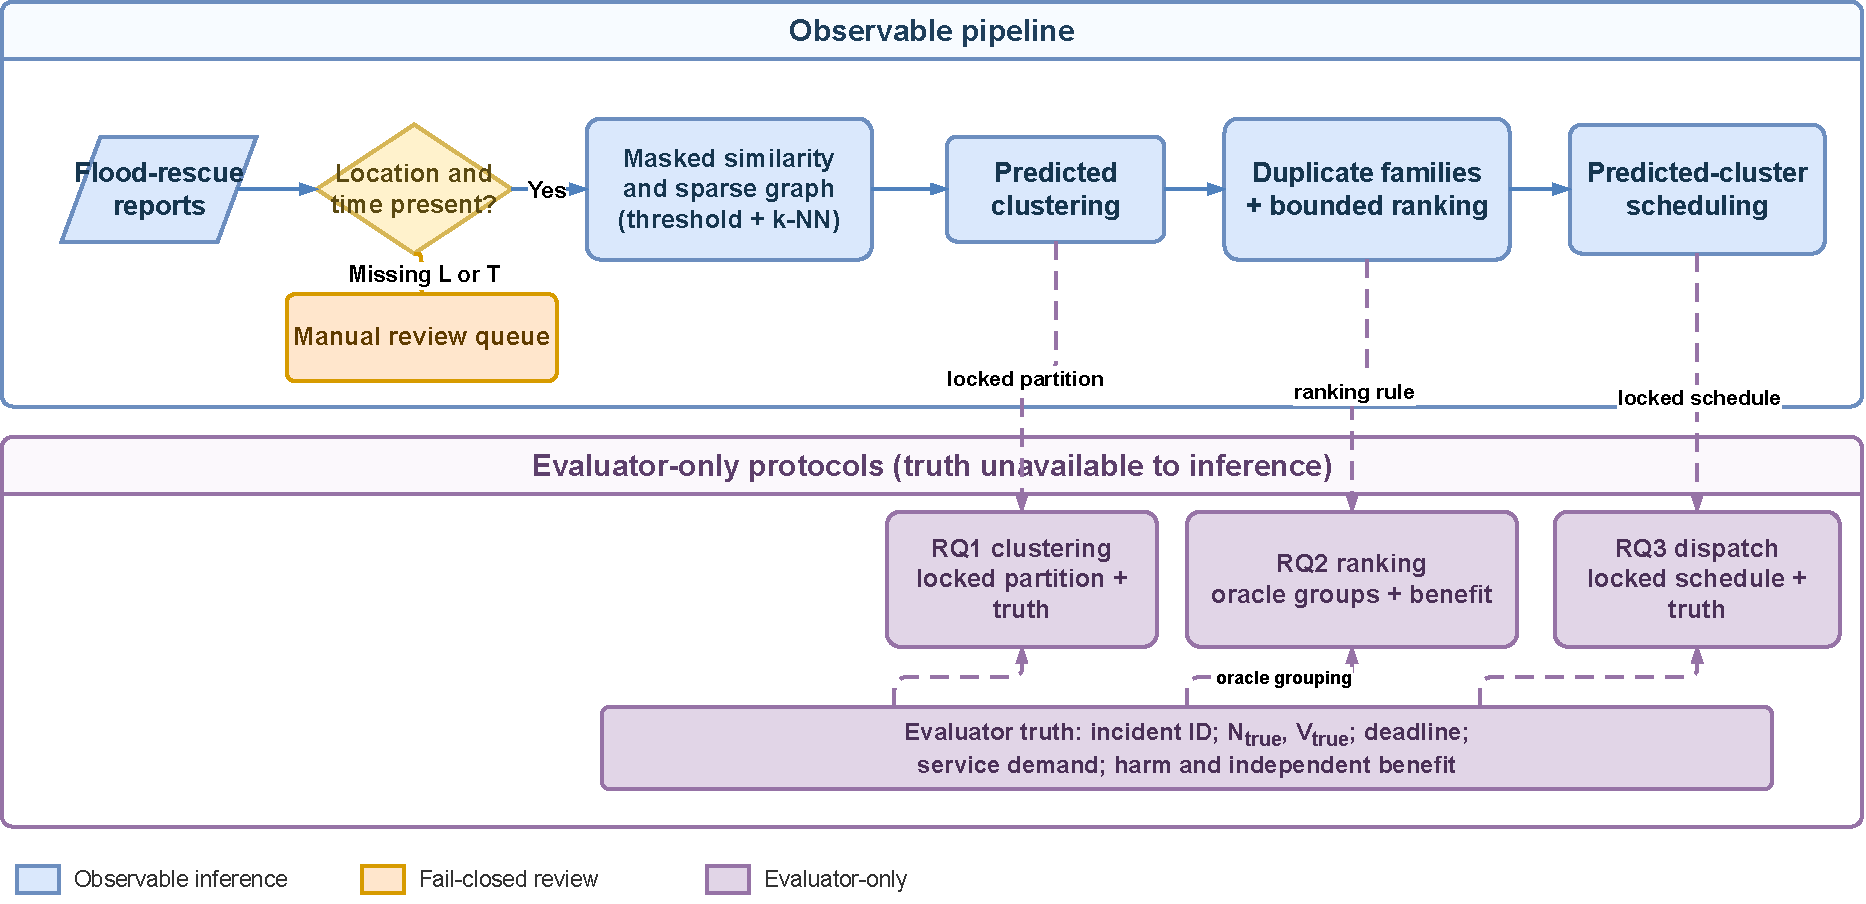
\includegraphics[width=\textwidth]{pipeline_v2.pdf}
\caption{Observable pipeline (solid), manual-review path (orange), and
evaluator-only truth join (dashed). The scheduler receives predicted clusters,
never incident truth.}
\label{fig:pipeline}
\end{figure}

Algorithms~\ref{alg:pipeline} and~\ref{alg:priority} restate admission,
graph construction, duplicate-aware scoring, and scheduling; neither receives
the evaluator-only truth join.

\subsection{Report Attributes and Missingness}

Each report is represented by the compact tuple
\[
r_i=(L_i,T_i,F_i,E_i,N_i,V_i,Q_i),
\]
where $L_i$ is a GPS location and $T_i$ is the observable report timestamp
(``created\_at''). Flood evidence $F_i$ and urgency evidence $E_i$ are in
$[0,1]$; $N_i\in\mathbb{Z}_{\geq0}$ is the reported trapped-person count;
$V_i\geq0$ is a vulnerability-evidence value; and $Q_i\in[0,1]$ is a
provenance/confidence heuristic. $Q_i$ is not a calibrated probability of
truth. The implementation also carries observable support fields such as
image presence, source type, province, and missing-field flags; these support
$Q_i$ and duplicate fingerprints but are not additional latent labels.

The score $Q_i$ is computed from observable image presence and the number of
nearby corroborating observable payloads (counted by unique payload identity)
using the proposed heuristic
\begin{equation}
\begin{aligned}
Q_i&=\operatorname{sigmoid}\!\left(b_0+b_1\mathbf{1}\{\text{image}_i\}
 +b_2\log(1+n_i^{\rm corrob})\right),\\[-1mm]
&(b_0,b_1,b_2)=(-.2,1.4,.9).
\end{aligned}
\label{eq:confidence}
\end{equation}
Here $\operatorname{sigmoid}(x)=(1+e^{-x})^{-1}$,
$\mathbf{1}\{\text{image}_i\}$ is one exactly when report $i$ contains an
image, and $n_i^{\rm corrob}\in\mathbb Z_{\geq0}$ counts distinct nearby
observable payloads. The dimensionless $b_0,b_1,b_2$ are the fixed intercept,
image, and corroboration coefficients; consequently $Q_i\in(0,1)$. This is a
pipeline rule, not a calibrated truth model. No independent receipt timestamp
or source family is assumed.

Following the general missing-variable kernel problem~\cite{smola2005missing},
we use the following fail-closed construction. The admission indicator
$a_i=\mathbf{1}\{L_i,T_i\text{ are observed}\}$.
Thus $a_i a_j=0$ prevents an edge involving a report whose geographic or
temporal separation is undefined; such a report follows the manual-review
path. Missing $F_i$ or $E_i$ is not zero-imputed: let
$I_F(i,j),I_E(i,j)\in\{0,1\}$ indicate that both reports contain the
corresponding observation and let
$m_{ij}=I_F(i,j)+I_E(i,j)$; then
\begin{equation}
C_{ij}=\frac{m_{ij}}{2}\exp\!\left[-I_F(i,j)\frac{|F_i-F_j|}{\tau_F}
-I_E(i,j)\frac{|E_i-E_j|}{\tau_E}\right],
\quad C_{ij}=0\ \text{if }m_{ij}=0.
\label{eq:context}
\end{equation}
$\tau_F,\tau_E>0$ are dimensionless flood- and urgency-difference scales, so
$C_{ij}\in[0,1]$. When $m_{ij}=2$, both contextual fields are used; when
$m_{ij}=1$, the
maximum contextual similarity is discounted to $1/2$; and when $m_{ij}=0$,
no contextual agreement is inferred. In the current 80-run artifact, every
report has location, event time, flood, and urgency. Hence $a_i=1$ and
$m_{ij}=2$ throughout the evaluated data, so Eq.~\ref{eq:context} uses its
full two-field exponential branch.
The missingness extension is specified and unit-tested, but missingness
robustness is not claimed as an empirical result of this benchmark.

\subsection{Similarity Graph and Derived Bounds}

For Haversine distance $d_{ij}$ and time difference $\Delta t_{ij}$, define
the Gaussian affinity~\cite{ng2001spectral} and exponential temporal decay
~\cite{zhou2013triggering}:
\begin{align}
G_{ij}&=\exp[-d_{ij}^{2}/(2\sigma^2)],&
T_{ij}&=\exp[-\Delta t_{ij}/\tau_t],\nonumber\\
w^\times_{ij}&=a_i a_jG_{ij}(\beta T_{ij}+\gamma C_{ij}),&
w^+_{ij}&=a_i a_j(\alpha G_{ij}+\beta T_{ij}+\gamma C_{ij}).
\label{eq:similarities}
\end{align}
$d_{ij}$ is measured in metres and $\Delta t_{ij}$ in minutes;
$\sigma>0$ and $\tau_t>0$ are the corresponding spatial and temporal
bandwidths. The dimensionless $G_{ij},T_{ij},C_{ij}\in[0,1]$ enter the product
and additive weights $w^\times_{ij}$ and $w^+_{ij}$ with nonnegative
$\alpha,\beta,\gamma$. Superscripts $\times$ and $+$ identify composition,
not multiplication or addition over report indices.
The exponential form is a precedent, not a claim that the complete
missingness-aware expression is copied from prior work~\cite{billot2008exponential}.
The product is a spatial gate motivated by spatial--range products such as
bilateral filtering~\cite{tomasi1998bilateral}; both compositions and all
weights here are defined by this paper.
The implementation forms the eligible pair matrix,
computes an empirical nonzero-weight quantile, removes weights at or below
that threshold, retains the endpoint-wise top-$k$ among the remaining directed
neighbours, and symmetrizes their union before community detection. Thus an
undirected node may have degree above $k$ when another node selects it.
Product and additive candidates are selected independently; the estimand is
therefore a pipeline comparison, not an operator-only causal effect. We treat
this independently calibrated contrast as the primary estimand for RQ1
because it asks whether each tuned pipeline provides a net empirical benefit.
Section~\ref{sec:results} also reports a matched-density contrast as a
secondary diagnostic. It reduces differences in retained-edge fraction and
mean degree, but different edge weights and memberships remain, so it does not
identify a causal effect of the composition operator.

\begin{theorem}[Product edge localization]
Let $B=\beta+\gamma>0$. If a product edge with threshold $0<\theta<B$ is
retained, then
$d_{ij}<\sigma\sqrt{2\log(B/\theta)}$. For $\theta\ge B$ the strict retained
set is empty; for $\theta\le0$ the threshold alone gives no finite cutoff.
\end{theorem}
\begin{proof}
Since $a_ia_j\le1$ and $T_{ij},C_{ij}\le1$,
$w^\times_{ij}\le B\exp[-d_{ij}^{2}/(2\sigma^2)]$. Combining
$\theta<w^\times_{ij}$ with positivity and taking logarithms gives the bound;
the endpoint cases follow from the same inequality.
\end{proof}
This is an edge statement. A component-diameter claim additionally needs a
bounded observed hop diameter; long transitive chains remain possible.

\begin{corollary}[Conditional component bound]
In the finite product region, a connected component with at least two nodes,
unweighted observed hop diameter $1\leq h<\infty$, and geographic diameter
$D$ satisfies $D<hr_\theta^\times$, where
$r_\theta^\times=\sigma\sqrt{2\log(B/\theta)}$. A singleton has $h=D=0$ and
is handled separately.
\end{corollary}
For a non-singleton, the result follows from the triangle inequality along a
path of at most $h$ retained edges. It is a conditional post-hoc component
bound, not an ex-ante compactness guarantee: the pipeline does not control
$h$.

For the additive form, assume $\alpha>0$. If
$B<\theta<B+\alpha$, every retained edge satisfies
\[
d_{ij}<r_\theta^+
=\sigma\sqrt{2\log\!\left(\frac{\alpha}{\theta-B}\right)}.
\]
If $\theta\ge B+\alpha$, the strict retained set is empty; if
$\theta\le B$, no non-trivial threshold-induced geographic cutoff exists in
general. Indeed, retention gives
$\theta<\alpha G_{ij}+\beta T_{ij}+\gamma C_{ij}\le\alpha G_{ij}+B$.
Thus product composition has a finite geographic edge bound throughout its
nonempty positive-threshold domain, whereas additive composition has such a
bound only above the maximum non-geographic contribution. Neither statement
alone implies better empirical clustering.

\Needspace*{0.62\textheight}
\begin{algorithm}[H]
\caption{Fail-closed observable report pipeline (Fig.~\ref{fig:pipeline})}
\label{alg:pipeline}
\begin{algorithmic}[1]
\footnotesize
\Require Reports $R=\{r_i\}$; kernel scales $\sigma,\tau_t,\tau_F,\tau_E$;
\Statex \hspace{2.5em}weights $\beta,\gamma$ (and $\alpha$ for the additive
composition); quantile $q$; neighbour cap $k$; Louvain/Leiden resolution $\rho$;
composition $m\in\{\text{product},\text{additive}\}$
\Ensure Dispatch schedule $S$; the algorithm below never reads incident
\Statex \hspace{2.5em}identity, benefit, deadline, or harm labels
\State $R_{\rm obs}\gets\emptyset$; $R_{\rm review}\gets\emptyset$
\For{each report $r_i\in R$}
    \State $a_i\gets\mathbf{1}\{L_i,T_i\text{ observed}\}$ \Comment{Section~2.1}
    \If{$a_i=0$}
        \State $R_{\rm review}\gets R_{\rm review}\cup\{r_i\}$
        \Comment{orange manual-review path}
    \Else
        \State $R_{\rm obs}\gets R_{\rm obs}\cup\{r_i\}$
    \EndIf
\EndFor
\State Compute $n_i^{\rm corrob}$ from unique payloads in $R_{\rm obs}$ and
set every $Q_i$ by Eq.~\ref{eq:confidence}
\State $E_0\gets$ \Call{BuildSimilarityEdges}{$R_{\rm obs},m$}
\Statex \hspace{2.5em}\textit{using the fixed scales and weights above}
\Statex \hspace{2.5em}\textit{BuildSimilarityEdges computes $G,T,C$ on the full eligible pair matrix}
\State $\theta\gets q$-quantile of the nonzero weights in $E_0$
\State $E_\theta\gets\{(i,j,w_{ij})\in E_0:w_{ij}>\theta\}$
\State $E^{\to}\gets\{(i,j,w_{ij})\in E_\theta:j\text{ is among }i\text{'s top-}k$
\Statex \hspace{2.5em}$\text{neighbours in }E_\theta\}$
\State $E\gets\{\{i,j\}: (i,j)\in E^{\to}\text{ or }(j,i)\in E^{\to}\}$
\State $\mathcal{G}\gets(R_{\rm obs},E)$
\State $\mathcal{C}\gets$ Louvain$/$Leiden$(\mathcal{G},\rho)$
\Comment{predicted clusters, never incident truth}
\For{each predicted cluster $C_k\in\mathcal{C}$}
    \State $P_k\gets$ \Call{PriorityScore}{$C_k$} \Comment{Algorithm~\ref{alg:priority}}
\EndFor
\State $S\gets$ Scheduler$(\{(C_k,P_k):C_k\in\mathcal{C}\})$
\Statex \hspace{2.5em}\textit{scheduler sees predicted clusters and $P_k$ only}
\State \Return $S$
\end{algorithmic}
\end{algorithm}

After $S$ is fixed, the offline evaluator may join $S$ and $R_{\rm review}$
with incident identity, benefit, deadline, and harm labels to compute ARI,
NDCG@5, and dispatch outcomes. This dashed path is not available to the
inference algorithm. In the current artifacts, the core schema requires
location and event time, so the manual-review branch is a fail-closed design
boundary rather than an empirically exercised missingness condition.

\subsection{Duplicate-Aware Bounded Ranking}

Exact duplicate payloads share a canonical fingerprint. Near duplicates are
joined by deterministic connected components under the observable envelope;
this transitive rule is not complete linkage. For a predicted cluster $C_k$,
let $\mathcal F_k$ denote the resulting exact/near-duplicate evidence
families inside that cluster. The revised estimator uses one confidence-gated
priority per cluster and family maxima so that overlapping reports are not
treated as disjoint people. Write
$\widetilde N_i=\min(N_i,N_{\rm ref})$ and
$\widetilde V_i=\min(V_i,V_{\rm cap})$ for the nonnegative clipped claims:
\begin{align}
\bar E_k&=\frac{\sum_{g\in\mathcal F_k}\max_{i\in g}Q_iE_i}
 {\max(1,\sum_{g\in\mathcal F_k}\max_{i\in g}Q_i)},&
\bar F_k&=\max_{g\in\mathcal F_k}\max_{i\in g}Q_iF_i,\nonumber\\
\bar N_k&=\min\!\left(1,\frac{\log(1+\max_{g\in\mathcal F_k}\max_{i\in g}Q_i\widetilde N_i)}
 {\log(1+N_{\rm ref})}\right),&
\bar V_k&=\max_{g\in\mathcal F_k}\max_{i\in g}Q_i\widetilde V_i,\nonumber\\
P_k&=\left[1+(\mu-1)\tanh(\bar V_k/s)\right]
 (\omega_E\bar E_k+\omega_F\bar F_k+\omega_N\bar N_k).
\label{eq:priority}
\end{align}
$g$ indexes an evidence family and $i\in g$ a report in that family.
$\bar E_k$ is a confidence-gated family aggregation, while $\bar F_k$,
$\bar N_k$, and $\bar V_k$ are respectively maximum flood, normalized clipped
population, and clipped vulnerability evidence. Here $N_{\rm ref}>0$ is the
population reference, $V_{\rm cap}\geq0$ the vulnerability cap, $s>0$ the
saturation scale, $1\leq\mu\leq2$ the maximum amplification, and
$\omega_E,\omega_F,\omega_N\geq0$ sum to one. Therefore
$\bar E_k,\bar F_k,\bar N_k\in[0,1]$, $\bar V_k\in[0,V_{\rm cap}]$, and
$0\leq P_k\leq\mu$.
The candidate source snapshot associated with the RQ2/RQ3 artifacts specifies
$\omega=(.34,.33,.33)$, $\mu=2$, $s=10$, $N_{\rm ref}=500$, and
$V_{\rm cap}=50$. Maxima limit duplicate multiplicity, the logarithm compresses
demand, clipping bounds individual evidence, and the hyperbolic tangent
saturates vulnerability amplification. Reliability-aware truth discovery
motivates $Q_i$ but does not derive these choices~\cite{wang2012truth}; they
still require sensitivity and expert validation
~\cite{tate2012vulnerability,gralla2014review}. Comparators test raw
multiplicity (legacy), single factors (urgency/population), an unbounded linear
score, chance ordering, and travel time (nearest-first); none is an endorsed
rescue policy.

\Needspace*{0.36\textheight}
\begin{algorithm}[H]
\caption{\textproc{PriorityScore}: duplicate-aware bounded priority (Eq.~\ref{eq:priority})}
\label{alg:priority}
\begin{algorithmic}[1]
\footnotesize
\Function{PriorityScore}{cluster $C_k$}
    \State $\mathcal F_k\gets$ exact-fingerprint groups and deterministic
    near-duplicate connected components within $C_k$
    \State Compute $\bar E_k,\bar F_k,\bar N_k,\bar V_k$ by Eq.~\ref{eq:priority}
    \State Compute $P_k$ by Eq.~\ref{eq:priority}
    \State \Return $P_k$
\EndFunction
\end{algorithmic}
\end{algorithm}

\section{Experimental Design}

\paragraph{Data contract and splits.}
The study uses two explicitly separated artifact suites. RQ1 uses the tracked
generator-3.0 bundle, a semi-synthetic dataset with geographic anchors from
the Copernicus EMSR848 Central Viet Nam activation~\cite{copernicusEMSR848};
Copernicus EMS, OpenStreetMap extracts, and the 2025 WorldPop constrained
population surface~\cite{worldpop2025vietnam} provide geographic or historical anchors, while
incidents, reports, duplicates, coordinated attacks, vulnerability, and
labels are synthetic. It contains 80 runs with 16 latent incidents and
26,288 reports (17,901 genuine, 3,587 duplicate, and 4,800 coordinated
nonincident reports), with 288--370 reports per run. Runs 1--20 are
development, 21--40 calibration, and 41--80 the test split held out from
calibration. These are within-generator tests, not mechanism-shift OOD
transfer.

RQ2 and RQ3 use a separately generated Candidate-4.1 bundle. This bundle is
a fully synthetic regional scenario defined by the generator and is not
claimed to be EMSR848-anchored. It contains 80 datasets, 16 incidents per
dataset, 30,229 reports in total, and 339--424 reports per dataset; the
development, calibration, and test seeds are 1000--1019, 2000--2019, and
3000--3039. Across its splits there are 1,554 fake reports and 2,560 labeled
duplicates (1,280 exact and 1,280 near). Each base dataset contains one
five-report coordinated high-confidence campaign and one report for each of
four low-confidence attack types; RQ2 stress scenarios perturb these inputs.
For both suites, inference reads only observable
\texttt{algorithm\_input.json}; ground truth is opened only after predictions
are fixed.

\begin{table}[t]
\centering\footnotesize
\setlength{\tabcolsep}{3pt}
\caption{Artifact construction. Geographic anchors do not make simulated
reports or outcomes into field observations.}
\label{tab:data-realism}
\begin{tabular}{p{.20\textwidth}p{.35\textwidth}p{.35\textwidth}}
\toprule
Layer & Generator 3.0 (RQ1) & Candidate 4.1 (RQ2/RQ3)\\
\midrule
Geographic context & EMSR848 context, OSM anchors, WorldPop cells
& Synthetic geometry; no EMSR848 claim\\
Reports/linkage & Synthetic incidents, reports, duplicates, campaigns, labels
& Synthetic incidents, reports, duplicates, attacks\\
Operational truth & Simulated need and vulnerability; population is not
trapped-person truth & Simulated benefit, deadlines, service, access, harm\\
External validity & Geographic plausibility only; no source snapshot or row
lineage & Controlled stresses; no field sample or transfer\\
\bottomrule
\end{tabular}
\end{table}

\paragraph{Fixed clustering stresses.}
The 40 held-out generator-3.0 test runs are also evaluated under seven fixed
conditions: the unmodified control; independent Gaussian location noise with
100 m or 300 m standard deviation on each local axis; independent Gaussian
timestamp noise with 15 min or 60 min standard deviation; and exact transport
copies at total multiplicity two or five, where only the observable report
identifier changes. Five configurations selected before this stress
evaluation are retained without tuning: Product Louvain, Additive Louvain,
matched-density Additive, Product Leiden, and geo-time DBSCAN. Each method
receives the same deterministic perturbation for a run and condition, yielding
$40\times7\times5=1{,}400$ fits. These controlled levels characterize the
tested pipeline and are not estimates of field measurement error or duplicate
prevalence.

\paragraph{Selection and comparators.}
The current notebook evaluates complete small grids on the 20 calibration
runs and selects mean ARI, breaking ties by standard deviation and canonical
configuration JSON. Product and additive use fixed $\tau_F=.25$,
$\tau_E=.35$, and $\beta=\gamma=.5$. The Product grid varies
$\sigma\in\{700,1200\}$ m, $\tau_t\in\{30,60\}$ min,
$q\in\{.90,.95\}$, and $k\in\{8,16\}$; the Additive grid varies
$\alpha\in\{1/3,1\}$, the same $\sigma,q,k$ sets, and fixes
$\tau_t=60$ min. Both fix resolution at $1.2$. Selected product Louvain uses
$\sigma=700$ m, $\tau_t=60$ min, quantile $.90$, $k=8$, and resolution $1.2$.
Selected additive Louvain uses $\alpha=1$, $\sigma=700$ m, $\tau_t=60$ min,
quantile $.95$, $k=8$, and resolution $1.2$. Because selected quantiles
differ, this is an independently calibrated pipeline comparison, not a
matched-density operator comparison. Comparators are convex similarity,
Product Leiden, geo-time DBSCAN, DBSCAN/HDBSCAN on scaled observable features,
spatial agglomeration, and coordinate K-means. Geo-time DBSCAN lacks
ST-DBSCAN's non-spatial criterion. Together these variants separate
composition and community detection, reduce the Product/Additive density
imbalance, and supply density-, hierarchy-, and geometry-based controls.

\paragraph{Endpoints and inference.}
ARI on incident-linked reports~\cite{hubert1985comparing} is the primary
endpoint; NMI, pairwise F1, geographic diameter, runtime, false destinations,
fake absorption, noise rejection, retained-edge fraction, and mean degree are
descriptive or operational diagnostics. RQ1 paired differences use 10,000
bootstrap resamples, Wilcoxon tests, and Holm correction; RQ2/RQ3 use 5,000
resamples. Reported p-values follow exported families. RQ1 adjusts all nine
Product-Louvain contrasts, with the product/additive/Leiden contrasts primary.
RQ2 adjusts three alignment endpoints within comparator and five robustness
endpoints within scenario; false-priority lift is descriptive. RQ3 adjusts 14
dispatch endpoints within each candidate/comparator/context block and
aggregates resource conditions within seed, retaining 40 pairs; the original
120 seed--condition analysis is diagnostic. RQ2 uses oracle groups to isolate
ranking, while RQ3 uses predicted clusters and independent simulated outcomes.

Fixed-stress ARI and pairwise F1 use original incident-linked reports so copy
multiplicities share an evaluation unit; all-payload and graph diagnostics are
descriptive. Each condition is paired with its method's control over 40 runs.
The 5,000-resample unadjusted CIs describe within-method change, not
between-method superiority.

\section{Results}
\label{sec:results}

\subsection{RQ1: Clustering Accuracy and Fixed Stresses}

Table~\ref{tab:clustering-results} reports the held-out clustering summary.
\begin{table}[!htbp]
\centering\scriptsize
\caption{RQ1 benchmark-test summary over 40 runs. Intervals are bootstrap
95\% confidence intervals; diameter is descriptive.}
\label{tab:clustering-results}
\begin{tabular}{lccr}
\toprule
Method & ARI [95\% CI] & Pair F1 & Mean diam. (km)\\
\midrule
Additive Louvain & .9191 [.8995,.9381] & .9247 & .3477\\
Product Leiden & .9165 [.8979,.9351] & .9223 & .3547\\
Convex Louvain & .9135 [.8940,.9320] & .9195 & .3547\\
Product Louvain & .9072 [.8864,.9271] & .9138 & .3585\\
Matched-density Additive & .8973 [.8763,.9175] & .9046 & .3743\\
Coordinate K-means & .8176 [.7976,.8384] & .8292 & .2977\\
Spatial agglomerative & .6235 [.5964,.6494] & .6506 & 4.1648\\
HDBSCAN & .5205 [.4565,.5811] & .5787 & 1.2527\\
Geo-time DBSCAN & .4978 [.4589,.5366] & .5450 & .6244\\
DBSCAN, all features & .4741 [.4273,.5201] & .5488 & .9340\\
\bottomrule
\end{tabular}
\end{table}

Additive Louvain has the highest mean ARI. Product minus independently tuned
Additive Louvain is $-0.01184$ with an unadjusted bootstrap CI
$[-0.02257,-0.00240]$, with 9 wins, 19 ties, and 12 losses. The Wilcoxon test
has raw $p=.0987$ and Holm-adjusted $p=.2560$; the interval and test use
different procedures, and the adjusted test does not establish a composition
advantage. Product minus matched-density Additive is $+0.00989$ with
unadjusted CI $[-0.00100,0.02082]$ and Holm-adjusted $p=.2560$; Product Leiden
versus Product Louvain has Holm-adjusted $p=.1120$. Product and matched-density
Additive have similar retained-edge fractions ($.03011$ and $.03021$) and mean
degrees (9.90 and 9.94), making their contrast a density diagnostic rather
than a causal estimate of the composition operator.

The product pipeline has zero fake absorption and zero fake rejection but a
16.49\% false-destination rate; fake reports avoid genuine destinations while
still forming fake-only destinations. This is an adverse operational result,
not evidence of misinformation robustness.

Figure~\ref{fig:rq1-fixed-stress} reports the fixed clustering stresses as
paired changes from each method's control. All tested location and timestamp
noise levels reduce mean ARI, and no method has the highest mean ARI in every
condition.

\begin{figure}[!htbp]
\centering
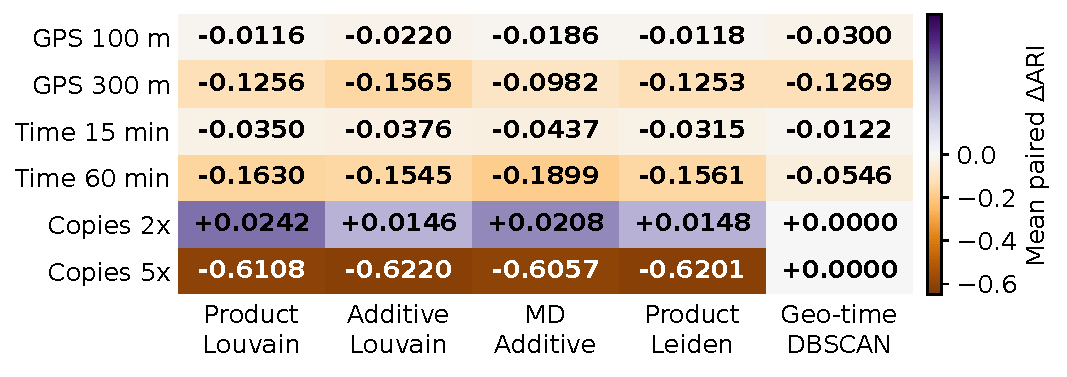
\includegraphics[width=.92\textwidth]{rq1_stress_delta_ari.pdf}
\caption{Mean paired change in RQ1 ARI relative to each method's control over
40 held-out runs. Cells use original incident-linked reports; negative values
indicate degradation; labels give control ARI, and zero change does not imply
high absolute accuracy. MD Additive denotes matched-density Additive.
Intervals are not shown and no between-method test is implied.}
\label{fig:rq1-fixed-stress}
\end{figure}

Twofold copies slightly increase ARI for all four graph variants, whereas
fivefold copies reduce their means to approximately $.30$; geo-time DBSCAN
remains at its lower control mean. These two tested multiplicities show a
non-monotone response, not a beneficial duplication effect or an identified
collapse threshold. For Product Louvain, the fivefold change is $-.6108$ with
an unadjusted paired-bootstrap 95\% CI $[-.6318,-.5881]$. Thresholding and
endpoint-wise top-$k$ sparsification are possible explanations, but the
protocol does not isolate a mechanism. An independent, unpooled rerun changes
only the aggregate twofold-copy graph values slightly; the GPS, timestamp,
fivefold-copy, and cross-condition conclusions remain unchanged. Thus
score-level invariance does not imply clustering invariance or end-to-end
robustness.

\subsection{RQ2: Copy Invariance and Benefit Alignment}

\begin{table}[!htbp]
\centering\scriptsize
\caption{RQ2 robustness means over the held-out Candidate-4.1 test split.
$n$ counts target-perturbation rows; $\Delta P$ is absolute normalized priority
drift, $\Delta r$ is normalized mean-rank drift, and churn is top-five churn.
R/L denote revised/legacy; lower is better.}
\label{tab:rq2-robustness}
\resizebox{\textwidth}{!}{%
\begin{tabular}{lrrrrrrr}
\toprule
Scenario & $n$ & $\Delta P_R$ & $\Delta P_L$ & $\Delta r_R$ & $\Delta r_L$ & Churn$_R$ & Churn$_L$\\
\midrule
Exact duplicate $2\times$ & 40 & .0000 & .0026 & .0000 & .0015 & .0000 & .0000\\
Exact duplicate $5\times$ & 40 & .0000 & .0086 & .0000 & .0046 & .0000 & .0100\\
Exact duplicate $10\times$ & 40 & .0000 & .0148 & .0000 & .0075 & .0000 & .0150\\
Near duplicate & 320 & .0016 & .0055 & .0004 & .0017 & .0006 & .0019\\
Contradictory $F/E$ & 40 & .0484 & .0611 & .0171 & .0290 & .0450 & .1100\\
Missingness/zero-imputation & 628 & .0063 & .0075 & .0019 & .0025 & .0029 & .0064\\
Low-confidence $E$ inflation & 40 & .0034 & .0012 & .0008 & .0006 & .0050 & .0000\\
Low-confidence $F$ inflation & 40 & .0026 & .0072 & .0000 & .0040 & .0000 & .0150\\
Low-confidence $N$ inflation & 40 & .0696 & .0140 & .0240 & .0071 & .0600 & .0150\\
Low-confidence $V$ inflation & 40 & .0758 & .0074 & .0263 & .0040 & .0500 & .0150\\
Coordinated high-confidence & 40 & .1688 & .0309 & .0175 & .0006 & .0350 & .0000\\
\bottomrule
\end{tabular}%
}
\end{table}

Under oracle incident grouping, revised NDCG@5 is .6669 (CI
[.6306,.7018]), Spearman is -.0304 (CI [-.1165,.0549]), and top-five overlap
is .285 (CI [.2349,.3400]). Revised exceeds legacy on NDCG@5 by .0121, but
the Holm-adjusted contrast is not significant. Its NDCG@5 point estimate is
lower than population-only (.6709) and random (.6763); these point estimates
do not by themselves establish significant differences. Because oracle
grouping removes upstream clustering errors from this RQ, the weak alignment
cannot be attributed solely to clustering.

Exact duplication at 2$\times$, 5$\times$, and 10$\times$ produces zero
revised priority drift when evidence grouping and inputs are fixed. A
coordinated high-confidence campaign instead produces drift .1688 and
false-priority lift .8828, increasing revised drift by .1379 relative to
legacy (Holm-adjusted $p\approx9.1\times10^{-12}$). Boundedness and
exact-copy invariance therefore do not guarantee ranking reliability.

Table~\ref{tab:rq2-robustness} expands the robustness audit beyond the two
headline cases. The revised score is invariant to exact-copy multiplicity and
usually changes less under near duplication, missingness, contradictory
evidence, and low-confidence flood inflation. Its bounded form is nevertheless
more sensitive than the legacy score to low-confidence urgency, population,
or vulnerability inflation and to coordinated high-confidence reports. These
are controlled synthetic perturbations, not estimates of attack prevalence or
field error.

Together, the oracle-group alignment and perturbation results separate narrow
invariance from empirical utility: exact-copy invariance holds under fixed
inputs, while benefit alignment remains unestablished.

\subsection{RQ3: Dispatch Outcomes}

After averaging the three resource scenarios within each seed, revised
priority on the Product partition increases simulated harm by 14.34 relative
to legacy while reducing the deadline-miss rate by 1.88 percentage points;
neither contrast is significant after Holm correction ($p=.563$ and
$p=.247$, respectively). Revised is worse than nearest-first on both harm
(Holm-adjusted $p=4.1\times10^{-5}$) and deadline misses (Holm-adjusted
$p=1.3\times10^{-6}$). Product is also worse than matched-density Additive
under revised priority on harm (Holm-adjusted $p=.000168$), and worse than
oracle on the corresponding outcomes. Predicted split, merge, and fake-only
destinations therefore have measurable scheduling consequences.

\begin{figure}[!htbp]
\centering
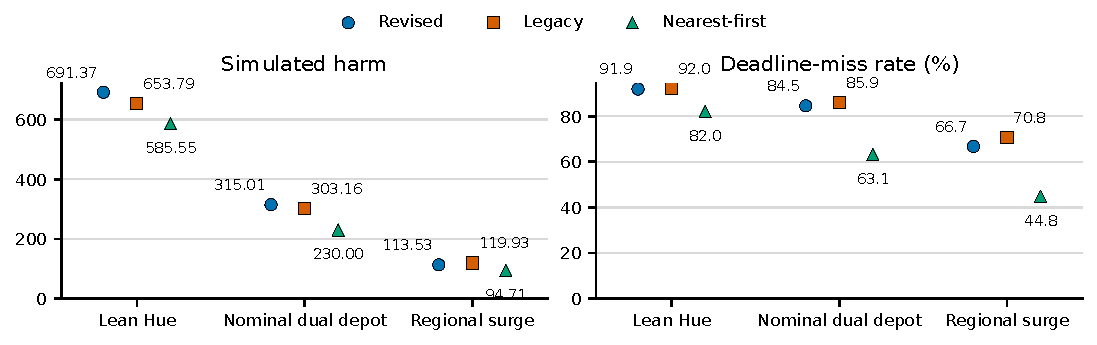
\includegraphics[width=\textwidth]{rq3_dispatch_conditions.pdf}
\caption{Descriptive Product-partition means over 40 test seeds for each
resource condition. Points are not additional independent samples or
between-policy tests. Primary inference averages the three conditions within
each seed and uses 40 seed-level pairs. Lower is better for both panels.}
\label{fig:rq3-dispatch}
\end{figure}

Figure~\ref{fig:rq3-dispatch} shows that nearest-first has lower mean harm and
deadline-miss rate in every tested condition. Revised priority lowers mean
deadline misses relative to legacy in the nominal and surge conditions and
lowers mean harm only in surge. One plausible explanation is that need-based
ranking does not fully represent travel costs and scheduling constraints, but
this experiment neither isolates that mechanism nor establishes
nearest-first as a field policy.

\subsection{Sensitivity of Heuristic Constants}
\label{sec:sensitivity}

To assess robustness to the fixed constants in $Q_i$ (Section~2.1) and $P$
(Eq.~\ref{eq:priority}), we define a local one-at-a-time sensitivity
analysis on the Candidate-4.1 ranking task. Each valid constant is perturbed
around its reference value while all other constants are held fixed, and
NDCG@5 is recomputed on the same 40 test seeds. The $\omega$ variants perturb
one component at a time and renormalize the vector; $\mu$ is restricted to its
policy-valid interval $[1,2]$. The locked rerun evaluates 21 configurations
on the same 40 held-out seeds, yielding 840 seed-level observations.
Table~\ref{tab:sensitivity} reports the tested levels and mean-NDCG@5 ranges;
no value is inferred from unrelated fixed-configuration comparisons.
\begin{table}[!htbp]
\centering\scriptsize
\caption{Candidate-4.1 one-at-a-time sensitivity of mean NDCG@5 to fixed
heuristic constants. Each range is the minimum--maximum mean over the tested
levels, including the reference level, on 40 test seeds. All spans are below
0.01 under the locked rerun.}
\label{tab:sensitivity}
\resizebox{\textwidth}{!}{%
\begin{tabular}{lccc}
\toprule
Constant & Reference/default value & Tested levels & Metric range\\
\midrule
$b_0$ ($Q_i$ intercept) & $-0.20$ & $[-0.24,-0.16]$ & $[.6653,.6672]$\\
$b_1$ (image weight) & $1.40$ & $[1.12,1.68]$ & $[.6669,.6687]$\\
$b_2$ (corroboration weight) & $0.90$ & $[0.72,1.08]$ & $[.6667,.6679]$\\
$\omega_E$ & $.34$ & component $\times\{.8,1,1.2\}$, renormalized & $[.6663,.6714]$\\
$\omega_F$ & $.33$ & component $\times\{.8,1,1.2\}$, renormalized & $[.6625,.6679]$\\
$\omega_N$ & $.33$ & component $\times\{.8,1,1.2\}$, renormalized & $[.6663,.6697]$\\
$\mu$ (vulnerability amplification) & $2$ & $\{1.6,1.8,2.0\}$ & $[.6644,.6683]$\\
$s$ (vulnerability saturation) & $10$ & $[8,12]$ & $[.6665,.6713]$\\
$N_{\rm ref}$ & $500$ & $[400,600]$ & $[.6669,.6669]$\\
$V_{\rm cap}$ & $50$ & $[40,60]$ & $[.6669,.6669]$\\
\bottomrule
\end{tabular}
}
\end{table}

All mean-NDCG@5 spans are below $.01$ over the tested levels; the largest is
$.00546$ for $\omega_F$. The unchanged reported mean for $N_{\rm ref}$ and
$V_{\rm cap}$ does not imply invariant per-seed scores or rankings. More
generally, local numerical stability coexists with weak benefit alignment and
does not validate the scoring rule or the constants outside these levels.

\section{Discussion and Threats to Validity}

The safeguards have stage-specific scope. Product gating gives a finite
conditional edge bound, yet no composition advantage is established and the
fixed stresses expose clustering sensitivity. The scheduler exposes
consequences of both imperfect destinations and an unvalidated ranking
objective. Clustering accuracy, score boundedness, and local parameter
stability answer distinct questions and cannot substitute for downstream
validation.

All data and outcomes are synthetic, and the separate RQ1 and RQ2/RQ3
generators do not test OOD transfer or field performance. RQ1 lacks an
empirical missingness test; the score lacks expert validation; and extraction,
deployment cost, source authenticity, and actual harm remain unmeasured.
Geographic anchors add context, but no raw snapshots, checksums, or row
lineage. Table~\ref{tab:data-realism} therefore documents construction, not
provenance or representativeness. These limits preclude policy or deployment
claims.

\section{Conclusion}

Product gating gives conditional edge-localization bounds, and family-wise
scoring is copy-invariant under fixed grouping and inputs. Neither ensures
clustering stability, benefit-aligned ranking, or better dispatch: fivefold
copies degrade graph clustering, ranking remains weak under oracle grouping,
and nearest-first has lower harm and deadline misses in every tested resource
condition. These endpoints require separate evaluation; clustering accuracy
and score boundedness are not downstream validation. Applicability remains
limited to the tested synthetic generators and configurations, without
establishing superiority, policy validity, or field readiness.

\section*{Data and Code Availability}

The Zenodo artifact~\cite{nguyen2026floodartifact} corresponds to
\href{https://github.com/ngthtrong/nckh2/releases/tag/v1.0.1}{GitHub Release
v1.0.1}. The RQ1 benchmark snapshot is
\href{https://github.com/ngthtrong/nckh2/commit/6ac75c202d04934deb46d84486132e54d42d735f}{\texttt{6ac75c2}};
the generator and external benchmark are at
\href{https://github.com/ngthtrong/nckh2/commit/a6be3e988dad1aa442c8c8e158c2bba96b2b7fb9}{\texttt{a6be3e9}}.
The public \href{https://github.com/ngthtrong/nckh2/tree/5fad10ddbe6e899769b59fe774850a41d2ac8d7d}{\texttt{clean} commit
\texttt{5fad10d}} adds primary fixed-stress results and an independent,
unpooled rerun. The primary notebook is included; the rerun notebook is
pending. These additions are outside \texttt{v1.0.1}; raw anchors are not
redistributed. Code is MIT licensed; the contribution follows the Springer
agreement, and other content retains its stated terms.

\begin{credits}
\subsubsection{\ackname} This study is funded by the Can Tho University, Code:
THS2026-68.

\subsubsection{\discintname} The authors have no competing interests to declare.
\end{credits}

\bibliographystyle{splncs04}
\bibliography{references}

\end{document}
